\input{header}

%\areaset[66pt]{415pt}{600pt}


\begin{document}
\title{WEKA Projekt}
\author{Fabian Langguth, Sebastian Koch}
\date{Wintersemester 10/11}

\maketitle

%TODO formatieren!
\section*{Aufgabe 1 Regellernen} 

F\"ur diese Aufgabe benutzen wir die Datens\"atze \emph{glass, iris} und \emph{splice}.
\emph{glass} wurde f\"ur den Prism-Learner mit dem Discretize-Filter verwendet (\emph{java weka.filters.supervised.attribute.Discretize -i glass.arff -o glass\_nom.arff -R 1,2,3,4,5,6,7,8,9 -c last}).

\textbf{Anzahl der Regeln}
\begin{table}[htb]
	\centering
\begin{tabular}{c|c|c|c}
	             & glass & iris & splice \\ \hline
Conjunctive Rule &   1   &  1   &   1    \\ \hline
JRip             &   8   &  4   &   14   \\ \hline
Prism	         &   63  &  16   &  3176    \\
\end{tabular}
\end{table}


\textbf{Gesamtanzahl der Bedingungen}
\begin{table}[htb]
	\centering
\begin{tabular}{c|c|c|c}
	             & glass & iris & splice \\ \hline
Conjunctive Rule &   2   &  1   &   1    \\ \hline
JRip             &  18   &  3   &   55   \\ \hline
Prism	         &  385  & 51   &   3176   \\
\end{tabular}
\end{table}


\textbf{Anzahl der vorhergesagten Klassen}
\begin{table}[htb]
	\centering
\begin{tabular}{c|c|c|c}
	             & glass & iris & splice \\ \hline
Conjunctive Rule &   1   &  1   &   1    \\ \hline
JRip             &   6   &  3   &   3    \\ \hline
Prism	         &   6   &  3   &   3    \\
\end{tabular}
\end{table}

\emph{Prism} erzeugt bei allen Datens\"atzen die meisten Regeln und Bedingungen. \emph{Conjunctive Rule} erzeugt fast immer nur eine Regel mit einer Bedingung.

Eine Default Rule existiert nur bei JRip. Dort wird als Defaultklasse \"ublicherweise die Klasse gew\"ahlt, die am h\"aufigsten im Datensatz vorkommt. Um zukünftige Daten zu klassifizieren ist das im Hinblick auf relative Häufigkeiten die sinnvollste Entscheidung.

Der Datensatz \emph{iris} l\"asst sich am einfachsten lernen, da man hier alle Algorithmen besonders wenig Regeln und besonders wenig Bedingungen ben\"otigen.

Auf dem Datensatz \emph{Contact Lenses} erzeugt \emph{JRip} 3 Regeln, wo bei einer davon der Default-Rule entspricht. \emph{Prism} erzeugt hingehen 9 Regeln. Die Anzahl der Bedingungen ist ebenfalls h\"oher f\"ur die von \emph{Prism} gefundenen Regeln. Daraus l\"asst sich folgern, dass \emph{JRip} vermutlich besser veralgemeinert. 
Dieser Unterschied entsteht hier vorallem durch dir verschiedenen Performance Ma\ss e. Da \emph{Prism} Precision verwendet, wird lediglich auf eine hohe Anzahl von korrekt klassifizierten Beispielen optimiert. Deshalb tendiert der Algorithmus eher zum Overfitting und erzeugt viele Regeln mit vielen Bedingungen. \emph{JRip} hingegen zieht durch das Gain Ma\ss\  auch die Anzahl der Regeln in Betracht und versucht dadurch nur wichtige Regeln zu lernen um Overfitting zu vermeiden.

\newpage

\section*{Aufgabe 2 Evaluation von Regellernern}

% TODO: Qualitaet einschaetzen

\begin{tabular}{c|c|c|c|c|c}
				Datensatz         & 1x5  & 1x10 & 1x20 & LOO  & Trainingsmenge   \\ \hline
				\emph{glass}      & 67.3 & 61.8 & 60.7 & 61.7 & 85.98   \\ \hline
				\emph{iris}       & 92.0 & 88.0 & 96.0 & 93.3 & 96.0    \\ \hline
				\emph{audiology}  & 67.3 & 66.4 & 69.9 & 69.9 & 76.1    \\ \hline
				\emph{ionosphere} & 89.2 & 92.0 & 90.0 & 89.2 & 100   \\ \hline
				\emph{yeast}      & 56.5 & 57.7 & 57.7 & 59.4 & 67.8   \\ \hline
\end{tabular}


% TODO: fuerht eine geschickte auswahl zu besseren abschaetzungen?

\begin{tabular}{c|c|c|c|c|c}
				Datensatz         & 10x10    \\ \hline
				\emph{glass}      & 67.3     \\ \hline
				\emph{iris}       & 92.0     \\ \hline
				\emph{audiology}  & 67.3     \\ \hline
				\emph{ionosphere} & 89.2     \\ \hline
				\emph{yeast}      & 56.5     \\ \hline
\end{tabular}


\begin{tabular}{c|c}
				Datensatz         & Validierungsmenge    \\ \hline
				\emph{glass}      & 73.1     \\ \hline
				\emph{iris}       & 93.3     \\ \hline
				\emph{audiology}  & 67.3   \\ \hline
				\emph{ionosphere} & 84.6   \\ \hline
				\emph{yeast}      & 56.1 \\ \hline
\end{tabular}

% TODO: wie war die abschaetzung?
% 10x10 Cross-Validation war grob am genausten
\newpage

\section*{Aufgabe 3 ROC-Kurven}
Datensatz: glass

\textbf{Fl\"ache unter ROC Kurve}
\begin{table}[htb]
	\centering
\begin{tabular}{c|c|c|c}
				Regellerner       & \emph{build wind float} & \emph{containers} & \emph{tableware}  \\ \hline
				\emph{J48}			& 0.81 & 0.87 & 0.93  \\ \hline
				\emph{Naive Bayes}  & 0.71 & 0.84 & 0.98  
\end{tabular}
\end{table}

\begin{figure}[htbp]
	\centering
		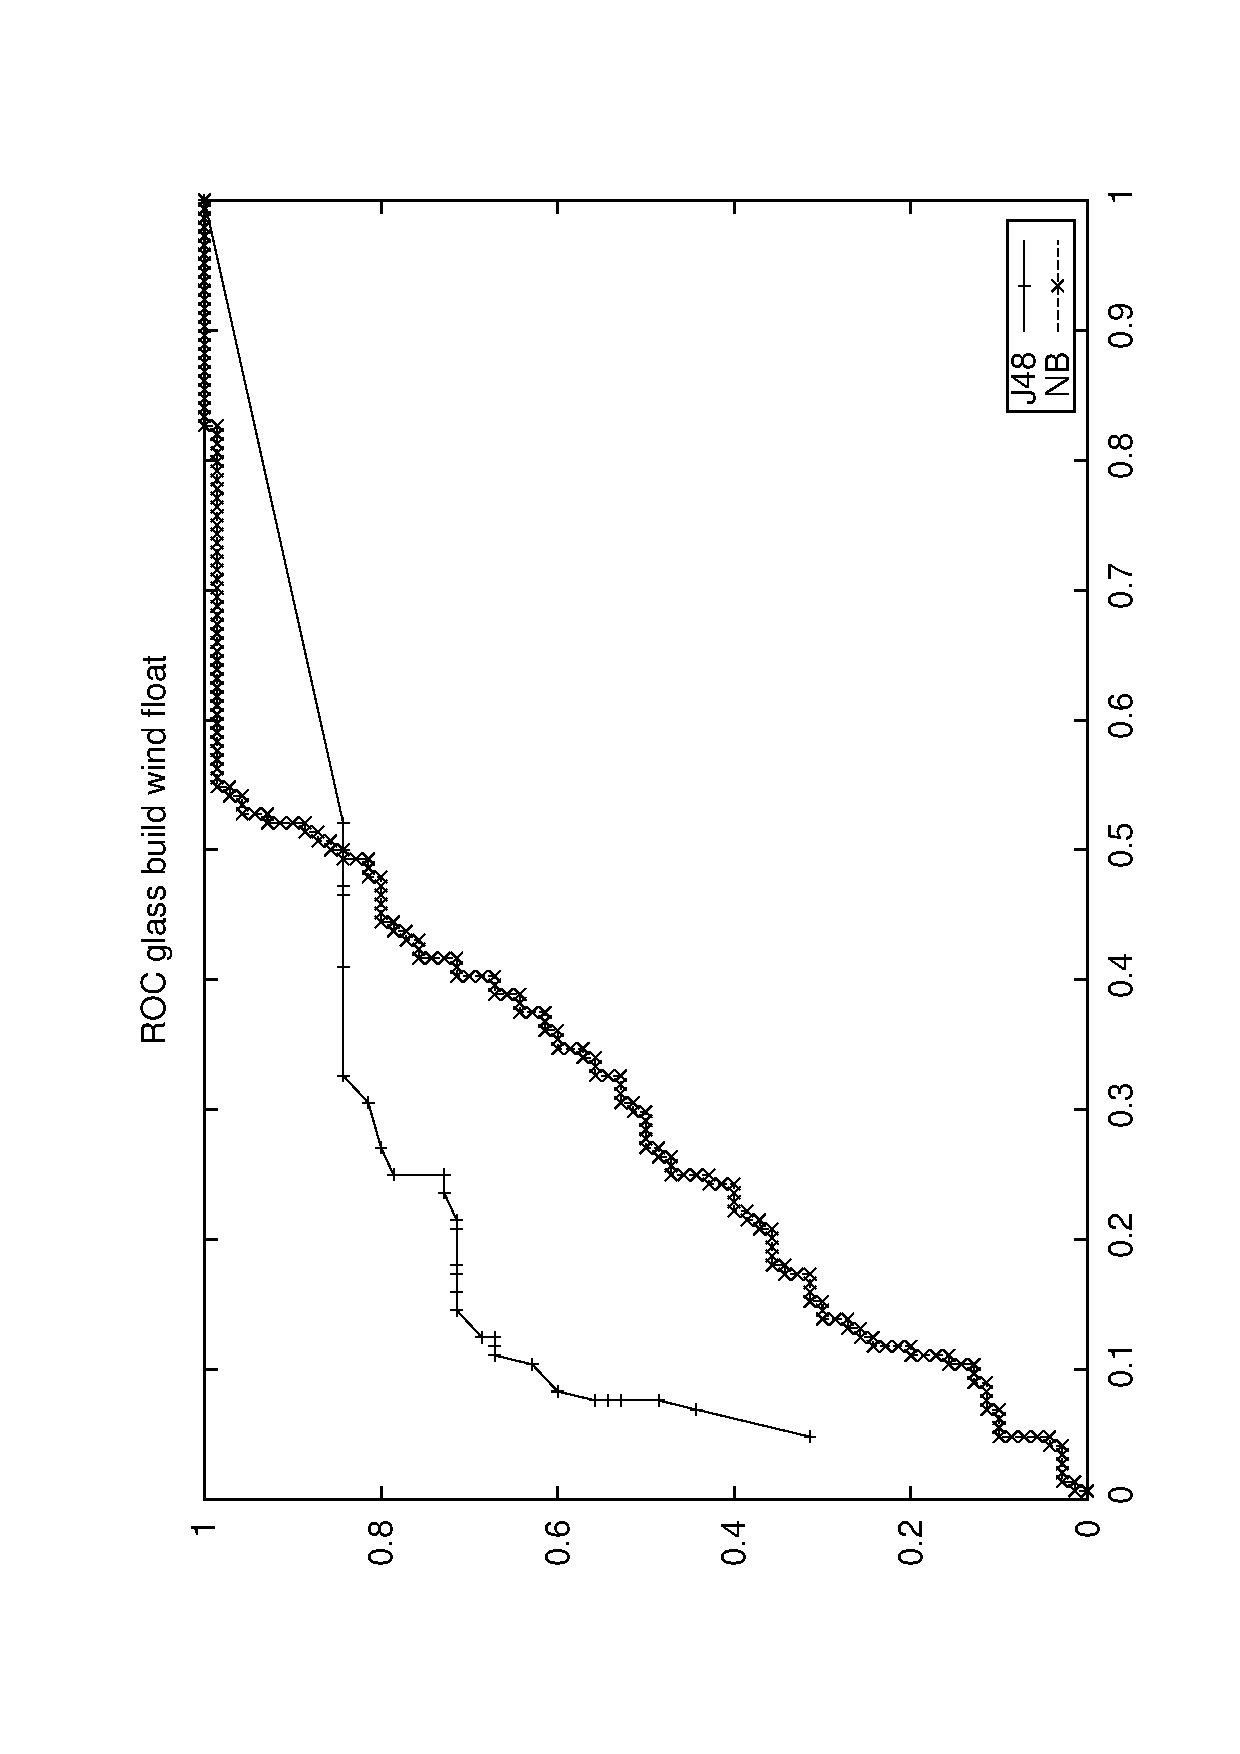
\includegraphics[height=3in]{pics/a3/ROC_glass_build_wind_float.pdf}
	\caption{ROC-Kurve f\"ur \emph{Naive Bayes} und \emph{J48} \"uber das Attribut \emph{build\_wind\_float}}
\end{figure}

\begin{figure}[htbp]
	\centering
		\includegraphics[height=3in]{pics/a3/ROC_glass_containers.pdf}
	\caption{ROC-Kurve f\"ur \emph{Naive Bayes} und \emph{J48} \"uber das Attribut \emph{containers}}
\end{figure}

\begin{figure}[htbp]
	\centering
		\includegraphics[height=3in]{pics/a3/ROC_glass_tableware.pdf}
	\caption{ROC-Kurve f\"ur \emph{Naive Bayes} und \emph{J48} \"uber das Attribut \emph{containers}}
\end{figure}

Bis auf wenige Klassen hat \emph{J48} eine h\"ohere Fl\"ache unter der ROC Kurve.
Anhand der ROC Kurven kann man also sagen, dass f\"ur eine uniforme Klassenverteilung und f\"ur eine Verteilung mit mehr negativen als positiven Beispielen \emph{J48} bessere Ergebnisse liefert. Bei Besonders vielen positiven Beispielen k\"onnte der Naive Bayes Klassifizierer bessere Ergebnisse erzielen.

\newpage
\section*{Aufgabe 4 Entscheidungsb\"aume}

Datens\"atz: glass (discretize filter), kr-vs-kp

\textbf{Area under ROC curve}
\begin{tabular}{c|c|c|c|c|c|c}
				Regellerner       & \emph{bwf} & \emph{bwn} & \emph{vwf}  & \emph{cont} & \emph{table} & \emph{head} \\ \hline
				\emph{J48 - unpruned}& 0.73 & 0.70 & 0.71 & 0.87 & 0.92 & 0.92 \\ \hline
				\emph{J48 - pruned}  & 0.77 & 0.73 & 0.73 & 0.86 & 0.87 & 0.84 \\ \hline
				\emph{ID3}           & 0.62 & 0.70 & 0.59 & 0.81 & 0.77 & 0.88 \\ \hline
\end{tabular}

Pruning hat nichts gebracht!

\begin{tabular}{c|c|c|c}
				Regellerner       & \emph{won} & \emph{nowin} \\ \hline
				\emph{J48 - unpruned} & 1.0 & 1.0  \\ \hline
				\emph{J48 - pruned}  & 1.0 & 1.0  \\ \hline
				\emph{ID3}  & 1.0 & 1.0 \\ \hline
\end{tabular}


\textbf{Accuracy}
\begin{tabular}{c|c|c}
				Regellerner       & \emph{glass} & \emph{kr-vs-kp}  \\ \hline
				\emph{J48 - unpruned}  & 57.94 & 99.41 \\ \hline
				\emph{J48 - pruned} & 57.94  & 99.44 \\ \hline
				\emph{ID3}  & 50.47 & 99.69\\ \hline
\end{tabular}

Gr\"osse der entstandenen B\"aume

\emph{glass}:
\begin{tabular}{c|c|c}
	Regellerner       & \emph{size of the tree} & \emph{number of leaves}  \\ \hline
	\emph{J48 - unpruned} & 221  & 199  \\ \hline
	\emph{J48 - pruned}   & 81   & 73   \\ \hline
	\emph{ID3}            & 550  & 496  \\ \hline
\end{tabular}


\emph{kr-vs-kp}:
\begin{tabular}{c|c|c}
	Regellerner       & \emph{size of the tree} & \emph{number of leaves}  \\ \hline
	\emph{J48 - unpruned}  & 82 & 43 \\ \hline
	\emph{J48 - pruned} & 59  & 31 \\ \hline
	\emph{ID3}  & 95 & 49\\ \hline
\end{tabular}

\newpage
\section*{Aufgabe 5 Nearest Neighbour}

Accuracy

\begin{tabular}{c|c|c}
                k-NN       & \emph{contact lenses} & \emph{kr-vs-kp}  \\ \hline
				\emph{k = 1} & 79.17  & 96.28  \\ \hline
				\emph{k = 3} & 79.17  & 96.50  \\ \hline
				\emph{k = 5} & 66.67  & 96.03  \\ \hline
				\emph{k = 7} & 58.33  & 95.40  \\ \hline
				\emph{k = 9} & 58.33  & 95.24  \\ \hline
				\emph{k = 11} & 58.33  & 95.06  \\ \hline
\end{tabular}

\newpage
\section*{Aufgabe 6 Regressionsb\"aume}


Tabelle f\"ur den \emph{Mean Absolute Error}:

\begin{table}
\begin{tabular}{c|c|c|c|c}
Datensatz  & \emph{R P MAE } & \emph{R U MAE} & \emph{M P MAE} & \emph{M U MAE} \\ \hline
\emph{auto-price}  & 2096.37 & 2075.07& 1403.20 & 1466.56 \\ \hline
\emph{concrete}    & 6.77    & 6.48   & 4.27    & 4.74     \\ \hline
\emph{housing}     & 3.29    & 3.20   & 2.39    & 2.50     \\ \hline
\emph{stock}       & 1.19    & 1.17   & 0.67    & 0.67     \\ \hline
\emph{winequality} & 0.55    & 0.53   & 0.51    & 0.55       
\end{tabular}
\caption{R: \emph{Regression-Trees} or M: \emph{Model-Trees} \\
U: \emph{unpruned} or P: \emph{pruned} }
\end{table}


Tabelle für den \emph{Root Mean Squared Error}:

\begin{table}
\begin{tabular}{c|c|c|c|c}
Datensatz  & \emph{R P RMSE} & \emph{R U RMSE} & \emph{M P RMSE} & \emph{M U RMSE} \\ \hline
\emph{auto-price}  & 3336.37  & 3287.12 & 2094.59 & 2171.16 \\ \hline
\emph{concrete}    & 8.68 & 8.33 & 5.89 & 6.36 \\ \hline
\emph{housing}     & 4.82 & 4.72 & 3.71 & 3.75 \\ \hline
\emph{stock}       & 1.60 & 1.59 & 0.93 & 0.94 \\ \hline
\emph{winequality} & 0.72 & 0.70 & 0.68 & 0.71   
\end{tabular}
\caption{R: \emph{Regression-Trees} or M: \emph{Model-Trees} \\
U: \emph{unpruned} or P: \emph{pruned} }
\end{table}


Aus den Tabellen k\"onnen wir ablesen, dass bei Regression-Tasks keine Verbesserung bringt. \emph{Model-Trees} haben auf allen Datensets einen kleineren Fehler als \emph{Regression-Trees}. Verwendet man Pruning bei \emph{Model-Trees} liefert es eine leichte Verbesserung.


\emph{M5P} liefert einen dem aus der \"Ubung \"ahnlichen Baum: Auf den ersten beiden Ebenen wird an denselben Attributen gesplittet. Danach erzeugt \emph{M5P} direkt Bl\"atter und l\"ost den Baum  nicht feiner auf. Der \emph{M5P}-Baum ist kleiner und wahrscheinlich allgemeiner. 

Der \emph{Root Mean Squared Error} des Baumes aus der \"Ubung betrugt $0.75$, der jetzt gelernte Baum hat einen \emph{RMSE} von $0.64$ auf den Testdaten. Dies best\"atigt unsere Vermutung, dass der \emph{M5P}-Baum allgemeiner ist.
\newpage
\section*{Aufgabe 7 Ensemble-Lernen}
Yeast:
Number of Leaves  : 	185

Size of the tree : 	369


Time taken to build model: 0.29 seconds

=== Stratified cross-validation ===
=== Summary ===

Correctly Classified Instances         831               55.9973 %
Incorrectly Classified Instances       653               44.0027 %
Kappa statistic                          0.4296
Mean absolute error                      0.1015
Root mean squared error                  0.2678
Relative absolute error                 65.2867 %
Root relative squared error             96.0945 %
Total Number of Instances             1484


Vowel:
Number of Leaves  : 	106

Size of the tree : 	198


Time taken to build model: 0.07 seconds

=== Stratified cross-validation ===
=== Summary ===

Correctly Classified Instances         807               81.5152 %
Incorrectly Classified Instances       183               18.4848 %
Kappa statistic                          0.7967
Mean absolute error                      0.0362
Root mean squared error                  0.1712
Relative absolute error                 21.8777 %
Root relative squared error             59.5369 %
Total Number of Instances              990     


vehicle:
Number of Leaves  : 	98

Size of the tree : 	195


Time taken to build model: 0.25 seconds

=== Stratified cross-validation ===
=== Summary ===

Correctly Classified Instances         613               72.4586 %
Incorrectly Classified Instances       233               27.5414 %
Kappa statistic                          0.6328
Mean absolute error                      0.1415
Root mean squared error                  0.3355
Relative absolute error                 37.7493 %
Root relative squared error             77.4887 %
Total Number of Instances              846


sick:
Number of Leaves  : 	34

Size of the tree : 	61


Time taken to build model: 0.08 seconds

=== Stratified cross-validation ===
=== Summary ===

Correctly Classified Instances        3727               98.807  %
Incorrectly Classified Instances        45                1.193  %
Kappa statistic                          0.8943
Mean absolute error                      0.0146
Root mean squared error                  0.1054
Relative absolute error                 12.685  %
Root relative squared error             43.9447 %
Total Number of Instances             3772     



abalone:
Number of Leaves  : 	1183

Size of the tree : 	2312


Time taken to build model: 0.75 seconds

=== Stratified cross-validation ===
=== Summary ===

Correctly Classified Instances         884               21.1635 %
Incorrectly Classified Instances      3293               78.8365 %
Kappa statistic                          0.1152
Mean absolute error                      0.0572
Root mean squared error                  0.2136
Relative absolute error                 89.3166 %
Root relative squared error            119.4373 %
Total Number of Instances             4177     


--------------------------------------------------------
yeast:
Bagging 10
Number of Leaves  : 	213

Size of the tree : 	425




Time taken to build model: 0.64 seconds

=== Stratified cross-validation ===
=== Summary ===

Correctly Classified Instances         902               60.7817 %
Incorrectly Classified Instances       582               39.2183 %
Kappa statistic                          0.4902
Mean absolute error                      0.0989
Root mean squared error                  0.2323
Relative absolute error                 63.5902 %
Root relative squared error             83.3597 %
Total Number of Instances             1484     

Bagging 20
Number of Leaves  : 	203

Size of the tree : 	405




Time taken to build model: 1.32 seconds

=== Stratified cross-validation ===
=== Summary ===

Correctly Classified Instances         905               60.9838 %
Incorrectly Classified Instances       579               39.0162 %
Kappa statistic                          0.4929
Mean absolute error                      0.0995
Root mean squared error                  0.2302
Relative absolute error                 63.9716 %
Root relative squared error             82.5918 %
Total Number of Instances             1484

Bagging 50

Number of Leaves  : 	208

Size of the tree : 	415




Time taken to build model: 3.71 seconds

=== Stratified cross-validation ===
=== Summary ===

Correctly Classified Instances         921               62.062  %
Incorrectly Classified Instances       563               37.938  %
Kappa statistic                          0.5071
Mean absolute error                      0.0997
Root mean squared error                  0.2287
Relative absolute error                 64.1179 %
Root relative squared error             82.0503 %
Total Number of Instances             1484     


Bagging 100
Number of Leaves  : 	219

Size of the tree : 	437




Time taken to build model: 6.79 seconds

=== Stratified cross-validation ===
=== Summary ===

Correctly Classified Instances         911               61.3881 %
Incorrectly Classified Instances       573               38.6119 %
Kappa statistic                          0.4976
Mean absolute error                      0.1   
Root mean squared error                  0.2289
Relative absolute error                 64.3026 %
Root relative squared error             82.1238 %
Total Number of Instances             1484



vowel:
bagging 10
Number of Leaves  : 	120

Size of the tree : 	200




Time taken to build model: 0.61 seconds

=== Stratified cross-validation ===
=== Summary ===

Correctly Classified Instances         895               90.404  %
Incorrectly Classified Instances        95                9.596  %
Kappa statistic                          0.8944
Mean absolute error                      0.045 
Root mean squared error                  0.1271
Relative absolute error                 27.2012 %
Root relative squared error             44.2289 %
Total Number of Instances              990

bagging 20
Number of Leaves  : 	127

Size of the tree : 	214




Time taken to build model: 1.78 seconds

=== Stratified cross-validation ===
=== Summary ===

Correctly Classified Instances         904               91.3131 %
Incorrectly Classified Instances        86                8.6869 %
Kappa statistic                          0.9044
Mean absolute error                      0.0458
Root mean squared error                  0.1236
Relative absolute error                 27.6877 %
Root relative squared error             43.0072 %
Total Number of Instances              990     


bagging 50
Number of Leaves  : 	118

Size of the tree : 	196




Time taken to build model: 2.68 seconds

=== Stratified cross-validation ===
=== Summary ===

Correctly Classified Instances         910               91.9192 %
Incorrectly Classified Instances        80                8.0808 %
Kappa statistic                          0.9111
Mean absolute error                      0.0461
Root mean squared error                  0.1219
Relative absolute error                 27.8727 %
Root relative squared error             42.3906 %
Total Number of Instances              990

bagging 100
Number of Leaves  : 	155

Size of the tree : 	244




Time taken to build model: 6.3 seconds

=== Stratified cross-validation ===
=== Summary ===

Correctly Classified Instances         916               92.5253 %
Incorrectly Classified Instances        74                7.4747 %
Kappa statistic                          0.9178
Mean absolute error                      0.0461
Root mean squared error                  0.1206
Relative absolute error                 27.89   %
Root relative squared error             41.96   %
Total Number of Instances              990     



vehicle:
bagging 10
Number of Leaves  : 	71

Size of the tree : 	141




Time taken to build model: 1.44 seconds

=== Stratified cross-validation ===
=== Summary ===

Correctly Classified Instances         648               76.5957 %
Incorrectly Classified Instances       198               23.4043 %
Kappa statistic                          0.688 
Mean absolute error                      0.143 
Root mean squared error                  0.2774
Relative absolute error                 38.1393 %
Root relative squared error             64.0837 %
Total Number of Instances              846

bagging 20
Number of Leaves  : 	83

Size of the tree : 	165




Time taken to build model: 1.76 seconds

=== Stratified cross-validation ===
=== Summary ===

Correctly Classified Instances         642               75.8865 %
Incorrectly Classified Instances       204               24.1135 %
Kappa statistic                          0.6786
Mean absolute error                      0.1452
Root mean squared error                  0.2749
Relative absolute error                 38.7456 %
Root relative squared error             63.4975 %
Total Number of Instances              846

bagging 50
Number of Leaves  : 	86

Size of the tree : 	171




Time taken to build model: 1.87 seconds

=== Stratified cross-validation ===
=== Summary ===

Correctly Classified Instances         645               76.2411 %
Incorrectly Classified Instances       201               23.7589 %
Kappa statistic                          0.6833
Mean absolute error                      0.1447
Root mean squared error                  0.2713
Relative absolute error                 38.595  %
Root relative squared error             62.671  %
Total Number of Instances              846

bagging 100
Number of Leaves  : 	78

Size of the tree : 	155




Time taken to build model: 4.61 seconds

=== Stratified cross-validation ===
=== Summary ===

Correctly Classified Instances         643               76.0047 %
Incorrectly Classified Instances       203               23.9953 %
Kappa statistic                          0.6801
Mean absolute error                      0.1448
Root mean squared error                  0.2707
Relative absolute error                 38.6168 %
Root relative squared error             62.5373 %
Total Number of Instances              846     



sick:
bagging 10
Number of Leaves  : 	31

Size of the tree : 	55




Time taken to build model: 1.64 seconds

=== Stratified cross-validation ===
=== Summary ===

Correctly Classified Instances        3724               98.7275 %
Incorrectly Classified Instances        48                1.2725 %
Kappa statistic                          0.8856
Mean absolute error                      0.0163
Root mean squared error                  0.092 
Relative absolute error                 14.1523 %
Root relative squared error             38.3619 %
Total Number of Instances             3772

bagging 20
Number of Leaves  : 	28

Size of the tree : 	49




Time taken to build model: 2.12 seconds

=== Stratified cross-validation ===
=== Summary ===

Correctly Classified Instances        3729               98.86   %
Incorrectly Classified Instances        43                1.14   %
Kappa statistic                          0.8978
Mean absolute error                      0.016 
Root mean squared error                  0.0882
Relative absolute error                 13.9227 %
Root relative squared error             36.8028 %
Total Number of Instances             3772


bagging 50
Number of Leaves  : 	31

Size of the tree : 	55




Time taken to build model: 2.92 seconds

=== Stratified cross-validation ===
=== Summary ===

Correctly Classified Instances        3729               98.86   %
Incorrectly Classified Instances        43                1.14   %
Kappa statistic                          0.8978
Mean absolute error                      0.0159
Root mean squared error                  0.0876
Relative absolute error                 13.7912 %
Root relative squared error             36.534  %
Total Number of Instances             3772     

bagging 100
Number of Leaves  : 	33

Size of the tree : 	59




Time taken to build model: 7.92 seconds

=== Stratified cross-validation ===
=== Summary ===

Correctly Classified Instances        3728               98.8335 %
Incorrectly Classified Instances        44                1.1665 %
Kappa statistic                          0.896 
Mean absolute error                      0.016 
Root mean squared error                  0.0879
Relative absolute error                 13.9057 %
Root relative squared error             36.6779 %
Total Number of Instances             3772     


abalone:
Bagging 10
Number of Leaves  : 	1077

Size of the tree : 	2097
Time taken to build model: 3.89 seconds

=== Stratified cross-validation ===
=== Summary ===

Correctly Classified Instances         964               23.0788 %
Incorrectly Classified Instances      3213               76.9212 %
Kappa statistic                          0.1319
Mean absolute error                      0.0575
Root mean squared error                  0.1799
Relative absolute error                 89.8126 %
Root relative squared error            100.6178 %
Total Number of Instances             4177     

Bagging 20
Number of Leaves  : 	1050

Size of the tree : 	2052

Time taken to build model: 7.53 seconds

=== Stratified cross-validation ===
=== Summary ===

Correctly Classified Instances         967               23.1506 %
Incorrectly Classified Instances      3210               76.8494 %
Kappa statistic                          0.1323
Mean absolute error                      0.0574
Root mean squared error                  0.1772
Relative absolute error                 89.7581 %
Root relative squared error             99.1077 %
Total Number of Instances             4177

Bagging 50
Number of Leaves  : 	1061

Size of the tree : 	2052




Time taken to build model: 20.06 seconds

=== Stratified cross-validation ===
=== Summary ===

Correctly Classified Instances         983               23.5336 %
Incorrectly Classified Instances      3194               76.4664 %
Kappa statistic                          0.1366
Mean absolute error                      0.0575
Root mean squared error                  0.1757
Relative absolute error                 89.7796 %
Root relative squared error             98.2396 %
Total Number of Instances             4177


Bagging 100
Number of Leaves  : 	1032

Size of the tree : 	2029




Time taken to build model: 44.37 seconds

=== Stratified cross-validation ===
=== Summary ===

Correctly Classified Instances         982               23.5097 %
Incorrectly Classified Instances      3195               76.4903 %
Kappa statistic                          0.1359
Mean absolute error                      0.0574
Root mean squared error                  0.1752
Relative absolute error                 89.7567 %
Root relative squared error             97.9418 %
Total Number of Instances             4177


--------- AdaBoost

yeast 
Number of Leaves  : 	203

Size of the tree : 	405


Weight: 1.61

Number of performed Iterations: 10


Time taken to build model: 0.69 seconds

=== Stratified cross-validation ===
=== Summary ===

Correctly Classified Instances         837               56.4016 %
Incorrectly Classified Instances       647               43.5984 %
Kappa statistic                          0.4363
Mean absolute error                      0.0876
Root mean squared error                  0.2743
Relative absolute error                 56.3424 %
Root relative squared error             98.4148 %
Total Number of Instances             1484


Number of Leaves  : 	222

Size of the tree : 	443


Weight: 1.68

Number of performed Iterations: 20


Time taken to build model: 1.42 seconds

=== Stratified cross-validation ===
=== Summary ===

Correctly Classified Instances         862               58.0863 %
Incorrectly Classified Instances       622               41.9137 %
Kappa statistic                          0.4556
Mean absolute error                      0.0841
Root mean squared error                  0.2772
Relative absolute error                 54.0385 %
Root relative squared error             99.4632 %
Total Number of Instances             1484

Number of Leaves  : 	237

Size of the tree : 	473


Weight: 1.79

Number of performed Iterations: 50


Time taken to build model: 4.38 seconds

=== Stratified cross-validation ===
=== Summary ===

Correctly Classified Instances         874               58.8949 %
Incorrectly Classified Instances       610               41.1051 %
Kappa statistic                          0.4667
Mean absolute error                      0.0829
Root mean squared error                  0.2835
Relative absolute error                 53.2977 %
Root relative squared error            101.703  %
Total Number of Instances             1484     
Number of Leaves  : 	215

Size of the tree : 	429


Weight: 1.57

Number of performed Iterations: 100


Time taken to build model: 8.03 seconds

=== Stratified cross-validation ===
=== Summary ===

Correctly Classified Instances         869               58.558  %
Incorrectly Classified Instances       615               41.442  %
Kappa statistic                          0.4624
Mean absolute error                      0.0827
Root mean squared error                  0.2848
Relative absolute error                 53.1493 %
Root relative squared error            102.1949 %
Total Number of Instances             1484

vowel

vehicle

sick 

abalone
\newpage
\section*{Aufgabe 8 Entdecken von Assoziationsregeln}

numerische attribute entfernt: fnlwgt, education-num

andere attribute entfernt: marital-status, capital-gain, capital-loss, sex

sortiert nach lift: 

relationship=Not-in-family 12583 ==> class=<=50K 11307    conf:(0.9) < lift:(1.18)> lev:(0.04) [1734] conv:(2.36)



numerische attribute entfernt: fnlwgt, education-num

andere attribute entfernt: marital-status, capital-gain, capital-loss, sex, age, relationship, native-country

sortiert nach confidence:

class=>50K 11687 ==> race=White 10607    conf:(0.91)

Da 85 \% der Teilnehmer der Studie race = white hatten, wurden sehr viele Regeln der Form ? => race = white gefunden. Entfernt man dieses Attribut, findet man interessantere Regeln.


attributes \u"brig: age, education, marital-status, occupation

1. age=0 9627 ==> marital-status=Never-married 8229    conf:(0.85)

2. age=3 8296 ==> marital-status=Married-civ-spouse 5139    conf:(0.62)


attributes: marital-status, relationship, class

class=>50K 11687 ==> marital-status=Married-civ-spouse 9984    conf:(0.85)

relationship=Own-child 7581 ==> class=<=50K 7470    conf:(0.99)





%TODO verschoenern
\newpage
\section*{Aufgabe 9  Pre-Processing}
Datensets: ionosphere, iris, yeast.

ionosphere non-filter:
Number of Leaves  : 	18

Size of the tree : 	35
=== Stratified cross-validation ===
=== Summary ===

Correctly Classified Instances         321               91.453  %
Incorrectly Classified Instances        30                8.547  %
Kappa statistic                          0.8096
Mean absolute error                      0.0938
Root mean squared error                  0.2901
Relative absolute error                 20.36   %
Root relative squared error             60.4599 %
Total Number of Instances              351

ionosphere filter:
Number of Leaves  : 	21

Size of the tree : 	27

=== Stratified cross-validation ===
=== Summary ===

Correctly Classified Instances         313               89.1738 %
Incorrectly Classified Instances        38               10.8262 %
Kappa statistic                          0.7571
Mean absolute error                      0.1333
Root mean squared error                  0.2969
Relative absolute error                 28.9567 %
Root relative squared error             61.8807 %
Total Number of Instances              351     


iris non-filter:
Number of Leaves  : 	5

Size of the tree : 	9

=== Stratified cross-validation ===
=== Summary ===

Correctly Classified Instances         144               96      %
Incorrectly Classified Instances         6                4      %
Kappa statistic                          0.94  
Mean absolute error                      0.035 
Root mean squared error                  0.1586
Relative absolute error                  7.8705 %
Root relative squared error             33.6353 %
Total Number of Instances              150     


iris filter:
Number of Leaves  : 	3

Size of the tree : 	4

=== Stratified cross-validation ===
=== Summary ===

Correctly Classified Instances         141               94      %
Incorrectly Classified Instances         9                6      %
Kappa statistic                          0.91  
Mean absolute error                      0.0598
Root mean squared error                  0.193 
Relative absolute error                 13.4523 %
Root relative squared error             40.9465 %
Total Number of Instances              150     



yeast non-filter:
Number of Leaves  : 	185

Size of the tree : 	369


=== Stratified cross-validation ===
=== Summary ===

Correctly Classified Instances         831               55.9973 %
Incorrectly Classified Instances       653               44.0027 %
Kappa statistic                          0.4296
Mean absolute error                      0.1015
Root mean squared error                  0.2678
Relative absolute error                 65.2867 %
Root relative squared error             96.0945 %
Total Number of Instances             1484     



yeast filter:
Number of Leaves  : 	64

Size of the tree : 	94

=== Stratified cross-validation ===
=== Summary ===

Correctly Classified Instances         877               59.097  %
Incorrectly Classified Instances       607               40.903  %
Kappa statistic                          0.4657
Mean absolute error                      0.1076
Root mean squared error                  0.239 
Relative absolute error                 69.1624 %
Root relative squared error             85.7568 %
Total Number of Instances             1484     



b)

ionosphere:
Number of Leaves  : 	21

Size of the tree : 	27


Time taken to build model: 0.02 seconds

=== Stratified cross-validation ===
=== Summary ===

Correctly Classified Instances         320               91.1681 %
Incorrectly Classified Instances        31                8.8319 %
Kappa statistic                          0.8043
Mean absolute error                      0.1185
Root mean squared error                  0.2769
Relative absolute error                 25.733  %
Root relative squared error             57.7242 %
Total Number of Instances              351     



iris:
Number of Leaves  : 	3

Size of the tree : 	4


Time taken to build model: 0 seconds

=== Stratified cross-validation ===
=== Summary ===

Correctly Classified Instances         140               93.3333 %
Incorrectly Classified Instances        10                6.6667 %
Kappa statistic                          0.9   
Mean absolute error                      0.0618
Root mean squared error                  0.2034
Relative absolute error                 13.8998 %
Root relative squared error             43.1411 %
Total Number of Instances              150     

=== Detailed Accuracy By Class ===

               TP Rate   FP Rate   Precision   Recall  F-Measure   ROC Area  Class
                 1         0          1         1         1          1        Iris-setosa
                 0.9       0.05       0.9       0.9       0.9        0.934    Iris-versicolor
                 0.9       0.05       0.9       0.9       0.9        0.939    Iris-virginica
Weighted Avg.    0.933     0.033      0.933     0.933     0.933      0.958

=== Confusion Matrix ===

  a  b  c   <-- classified as
 50  0  0 |  a = Iris-setosa
  0 45  5 |  b = Iris-versicolor
  0  5 45 |  c = Iris-virginica

yeast
Number of Leaves  : 	64

Size of the tree : 	94


Time taken to build model: 0.02 seconds

=== Stratified cross-validation ===
=== Summary ===

Correctly Classified Instances         846               57.0081 %
Incorrectly Classified Instances       638               42.9919 %
Kappa statistic                          0.4369
Mean absolute error                      0.1125
Root mean squared error                  0.2444
Relative absolute error                 72.3218 %
Root relative squared error             87.6814 %
Total Number of Instances             1484     





----------------------

letter:
a)
Number of Leaves  : 	1226

Size of the tree : 	2451


Time taken to build model: 4.23 seconds

=== Stratified cross-validation ===
=== Summary ===

Correctly Classified Instances       17596               87.98   %
Incorrectly Classified Instances      2404               12.02   %
Kappa statistic                          0.875 
Mean absolute error                      0.0105
Root mean squared error                  0.0903
Relative absolute error                 14.2446 %
Root relative squared error             46.9362 %
Total Number of Instances            20000     


Number of Leaves  : 	9624

Size of the tree : 	10520


Time taken to build model: 0.36 seconds

=== Stratified cross-validation ===
=== Summary ===

Correctly Classified Instances       15725               78.625  %
Incorrectly Classified Instances      4275               21.375  %
Kappa statistic                          0.7777
Mean absolute error                      0.0184
Root mean squared error                  0.1145
Relative absolute error                 24.8961 %
Root relative squared error             59.5544 %
Total Number of Instances            20000

b)
Number of Leaves  : 	9624

Size of the tree : 	10520


Time taken to build model: 1 seconds

=== Stratified cross-validation ===
=== Summary ===

Correctly Classified Instances       15733               78.665  %
Incorrectly Classified Instances      4267               21.335  %
Kappa statistic                          0.7781
Mean absolute error                      0.0184
Root mean squared error                  0.1146
Relative absolute error                 24.8632 %
Root relative squared error             59.5869 %
Total Number of Instances            20000

segment:
a)
Number of Leaves  : 	39

Size of the tree : 	77


Time taken to build model: 0.09 seconds

=== Stratified cross-validation ===
=== Summary ===

Correctly Classified Instances        2239               96.9264 %
Incorrectly Classified Instances        71                3.0736 %
Kappa statistic                          0.9641
Mean absolute error                      0.0104
Root mean squared error                  0.0914
Relative absolute error                  4.2494 %
Root relative squared error             26.1312 %
Total Number of Instances             2310     


Number of Leaves  : 	295

Size of the tree : 	324


Time taken to build model: 0.01 seconds

=== Stratified cross-validation ===
=== Summary ===

Correctly Classified Instances        2202               95.3247 %
Incorrectly Classified Instances       108                4.6753 %
Kappa statistic                          0.9455
Mean absolute error                      0.0175
Root mean squared error                  0.1067
Relative absolute error                  7.1348 %
Root relative squared error             30.4966 %
Total Number of Instances             2310

b)

Number of Leaves  : 	295

Size of the tree : 	324


Time taken to build model: 0.05 seconds

=== Stratified cross-validation ===
=== Summary ===

Correctly Classified Instances        2177               94.2424 %
Incorrectly Classified Instances       133                5.7576 %
Kappa statistic                          0.9328
Mean absolute error                      0.0198
Root mean squared error                  0.1165
Relative absolute error                  8.0774 %
Root relative squared error             33.2926 %
Total Number of Instances             2310     




\end{document}
